\documentclass[10pt,a4paper]{report}
\usepackage[utf8]{inputenc}
\usepackage{amsmath}
\usepackage{amsfonts}
\usepackage{amssymb}
\usepackage{graphicx}
\begin{document}
\title{English/Spanish Translation \\ with Language Identification - \\ Project Milestone}
\author{Alex Shah}
\date{11/12/17}

\maketitle

\section{Abstract}
This project's goal is to combine different architectures of neural networks to form a functional English/Spanish translator with the ability to detect the input language and translate to the corresponding opposite language. The resulting product combines a network to classify the input language with a sequence to sequence based recurrent neural networks for creating contextually aware translations.
\clearpage

\section{Introduction}

\subsection{Language Classification}
Classifying a given input is handled by a Convolutional Neural Network (CNN). It is crucial to quickly determine the input language as identifying the language is an intermediary step before translation. However, incorrectly determining the input language will create incorrect translations. Therefore it is important that the classification network is able to quickly but accurately detect the input language.

\subsection{Contextually Aware Translation}
Strides have been made using deep learning and deep network models for Machine Translation (MT) accuracy, making MT ever more accurate in contextually aware translation. Sequence to Sequence networks (Seq2Seq) are built like an encoder/decoder. The encoded input text is examined to determine the decoded output in the target language. An attention mechanism is used to limit the amount of backward and forward information sharing. Too much or too little information while determining context can have adverse effects on translation. 

Neural Machine Translation (NMT) is a specifically derivated method of Seq2Seq focusing on accuracy and efficiency of training translation models.
\clearpage

\begin{figure}
\begin{center}
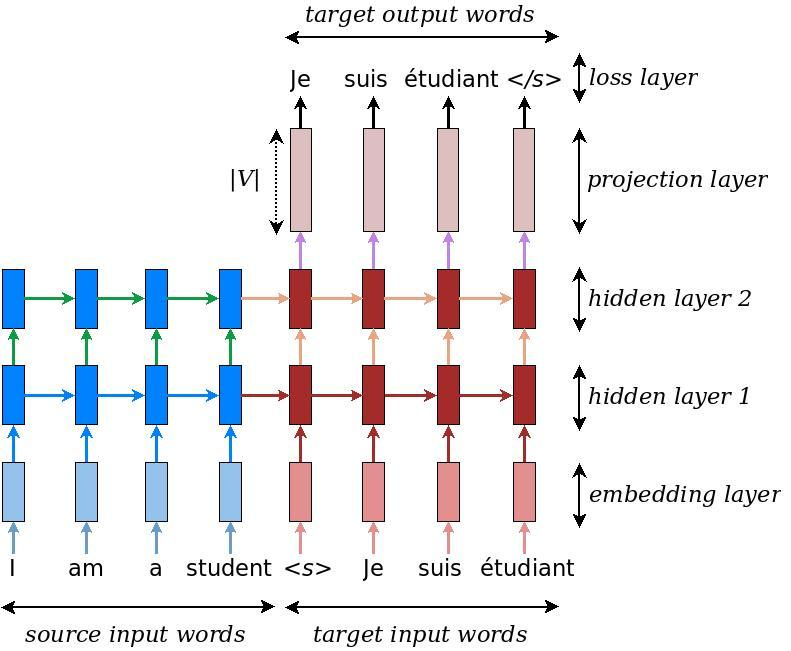
\includegraphics[width=0.8\textwidth]{seq2seq.jpg}
\caption{Sequence to Sequence Model (Luong, 2017)}
\end{center}
\end{figure}

\begin{figure}
\begin{center}
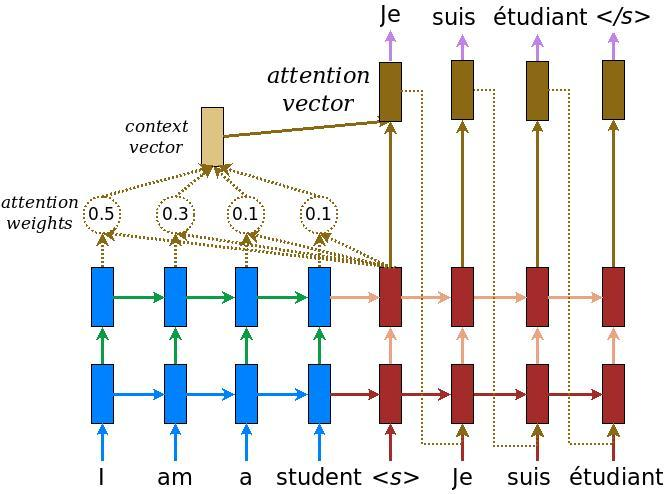
\includegraphics[width=0.8\textwidth] {attention_mechanism.jpg}
\caption{Sequence to Sequence Model with Attention Mechanism (Luong, 2017)}
\end{center}
\end{figure}

\clearpage
\section{Datasets and Training}
NLTK
Statmt - European parliament - En-Es

Train Classifier; Train translation both ways at once

\section{References}
\subsection{Resources}

https://github.com/tensorflow/nmt

https://github.com/google/seq2seq

http://www.nltk.org/

\subsection{Articles}

https://nlp.stanford.edu/projects/nmt/

https://research.googleblog.com/2017/07/building-your-own-neural-machine.html

https://sites.google.com/site/acl16nmt/

https://github.com/lmthang/thesis

https://google.github.io/seq2seq/data/


\subsection{Papers}

https://arxiv.org/pdf/1611.04558v1.pdf

https://papers.nips.cc/paper/5346-sequence-to-sequence-learning-with-neural-networks.pdf

http://aclweb.org/anthology/D/D14/D14-1179.pdf

https://arxiv.org/pdf/1409.0473.pdf

https://arxiv.org/pdf/1508.04025.pdf

https://arxiv.org/abs/1609.08144

https://arxiv.org/abs/1703.01619


\subsection{Data}

http://www.statmt.org/europarl/

https://conferences.unite.un.org/UNCorpus

http://www.statmt.org/wmt17/translation-task.html


\end{document}